Since the core of the programming was provided to us in the skeleton code to add new features, I used the pre-existing code and designed and built the additional features based on it. Firstly, I developed separate files called attack.c, emeny.c, and menu.c for the three primary new features. I made some other adjustments after adding it to the commons header file and the struct file. 

\subsection{New Maps or Levels}
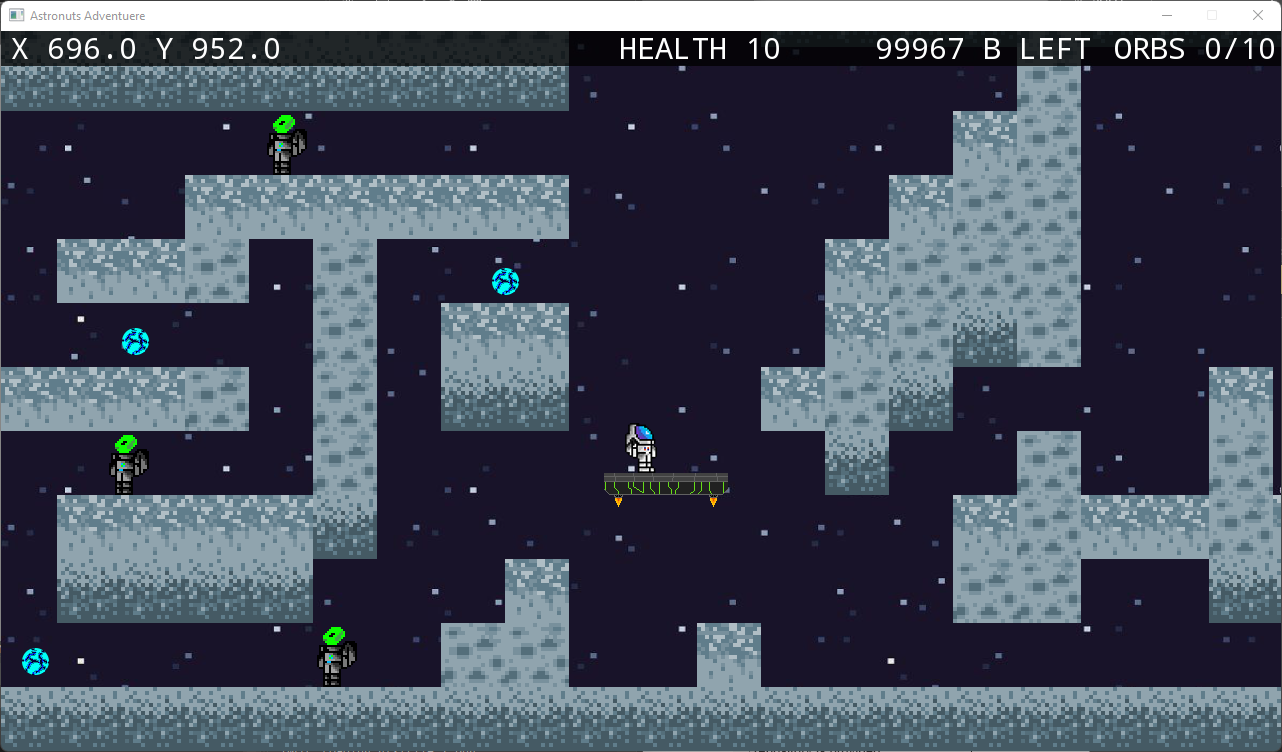
\includegraphics[width=1\linewidth]{images/ss.png}
We were provided a single map in the skeleton code. These were set up using a 40 by 60 number matrix ranging from 1 to 7. The initmap function then read this by calling the io.c file. The map was created, and the entities from the entX.dat folder were placed depending on their coordinates.
These files served as the foundation for the additional four maps I produced. Similarly, to the maps, I had to create four more entity files to add the entities to the new maps. The Alien entity was also updated to be able to be added using this method. during the map making process I found it difficult to determine the correct coordinates while creating the map, so I used the drawText method to print out the players' x and y coordinates. This, however, was solely for development and testing and will be deleted in the final version.


\subsection{Game Textures and theme}

\begin{tabular}{ll}
    Astronaut Right Still & 
\includegraphics[width=.08\linewidth]{C:/Users/ru4en/OneDrive/Desktop/SpringProjectx/gfx/astroF1.png} \\
    Astronaut Left Still & 
\includegraphics[width=.08\linewidth]{C:/Users/ru4en/OneDrive/Desktop/SpringProjectx/gfx/astroB1.png} \\
    Astronaut Right Walk & 
\includegraphics[width=.08\linewidth]{C:/Users/ru4en/OneDrive/Desktop/SpringProjectx/gfx/astroF2.png} \\
    Astronaut Left Walk & 
\includegraphics[width=.08\linewidth]{C:/Users/ru4en/OneDrive/Desktop/SpringProjectx/gfx/astroB2.png} \\
    Astronaut Right Jump & 
\includegraphics[width=.08\linewidth]{C:/Users/ru4en/OneDrive/Desktop/SpringProjectx/gfx/astroFJ.png} \\
    Astronaut Left Jump & 
\includegraphics[width=.08\linewidth]{C:/Users/ru4en/OneDrive/Desktop/SpringProjectx/gfx/astroBJ.png} \\
\end{tabular}
\begin{tabular}{ll}
    Alien Right Still & 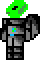
\includegraphics[width=.08\linewidth]{C:/Users/ru4en/OneDrive/Desktop/SpringProjectx/gfx/alienB1.png} \\
    Alien Left Still & 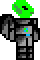
\includegraphics[width=.08\linewidth]{C:/Users/ru4en/OneDrive/Desktop/SpringProjectx/gfx/alienF1.png} \\
    Rock 1 & 
\includegraphics[width=.08\linewidth]{C:/Users/ru4en/OneDrive/Desktop/SpringProjectx/gfx/rock1.png} \\   
    Rock 2 & 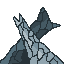
\includegraphics[width=.08\linewidth]{C:/Users/ru4en/OneDrive/Desktop/SpringProjectx/gfx/rock2.png} \\
    Lazar Shot & 
\includegraphics[width=.08\linewidth]{C:/Users/ru4en/OneDrive/Desktop/SpringProjectx/gfx/shot.png} \\
    Orb & 
\includegraphics[width=.08\linewidth]{C:/Users/ru4en/OneDrive/Desktop/SpringProjectx/gfx/spr.png} \\
    Moon Topsoil & 
\includegraphics[width=.08\linewidth]{C:/Users/ru4en/OneDrive/Desktop/SpringProjectx/gfx/tile_1.png} \\
    Moon Rock & 
\includegraphics[width=.08\linewidth]{C:/Users/ru4en/OneDrive/Desktop/SpringProjectx/gfx/tile_2.png} \\
    Moon Bedrock & 
\includegraphics[width=.08\linewidth]{C:/Users/ru4en/OneDrive/Desktop/SpringProjectx/gfx/tile_3.png}
\end{tabular}

The controls to the player are listened for in the game loop once the game starts. To interact with the game, the user can then move, shoot, or jump using W A S D Right Shift or spacebar. If the player gathers all of the orbs on the map, the game finishes, and the level is completed. If the player touches the alien, it loses health, and if it falls below zero, the game terminates, and the player is returned to the menu. This is visualized using the flowchart below.



The game, as indicated in the introduction, is based on a shooting game with a moon theme. I choose pixel art as the art style for this game. All of the textures in the game were created in Photoshop using a certain colour palette and aspect ratio. The player includes six distinct texture pictures for the left and right positions of the three functions it may perform: stand, walk, and leap. Similarly, the alien had textures on both the left and right sides. The platform was designed to seem like an industrial Si-Fi spaceship platform. Three tiles were made with topsoil, dirt, and bedrock designs to make the terrain look like the moon. Rocks were added for astatic, and the pizza was also changed to a blue orb to fit the theme.

\subsection{Game Menu}
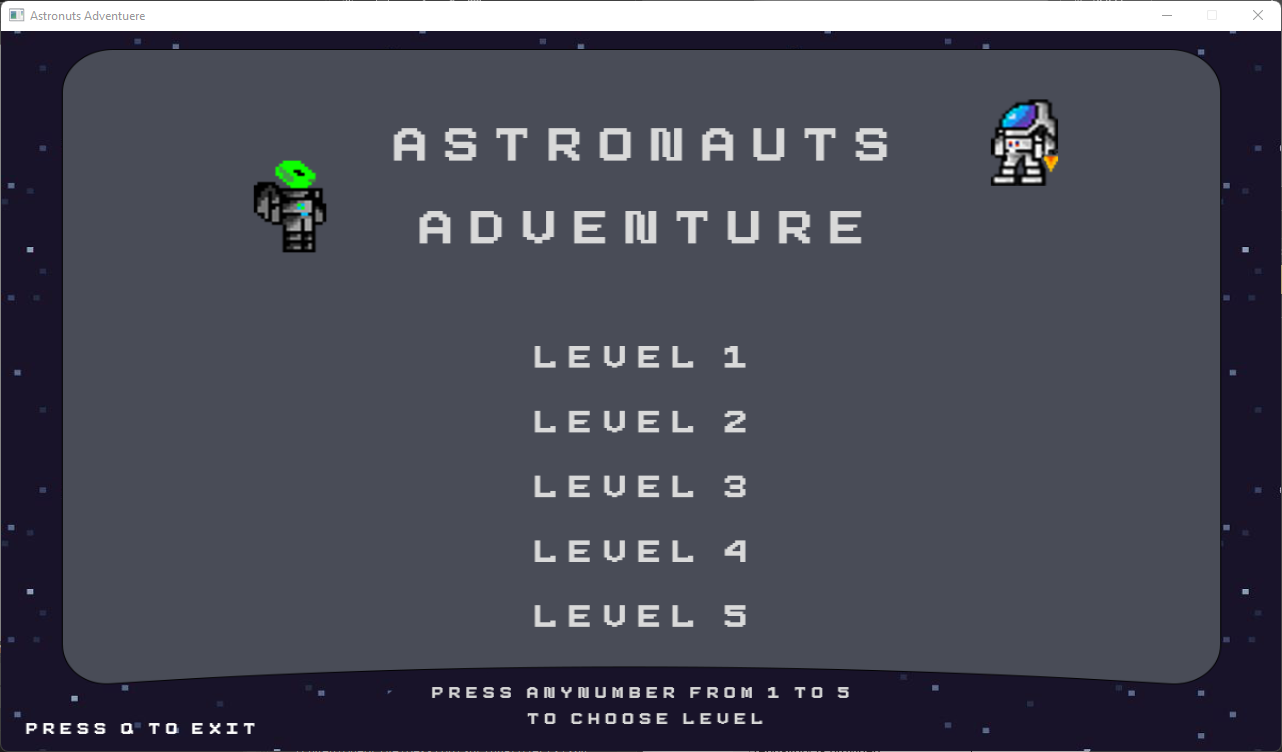
\includegraphics[width=1\linewidth]{images/ss5.png}
The game menu is comprised of a basic backdrop image created in Photoshop. In the same way as the game does, this loops until any number from 1 to 5 is pressed to begin the level. Alternatively, Q could be pressed to exit the application. Players may also return to this menu by pressing esc during the game, although their progress will be lost. 

\lstinputlisting[language=c]{C:/Users/ru4en/OneDrive/Desktop/SpringProjectx/src/menu.c}

 \newpage

 \subsection{Player Attacks (Shooting)}
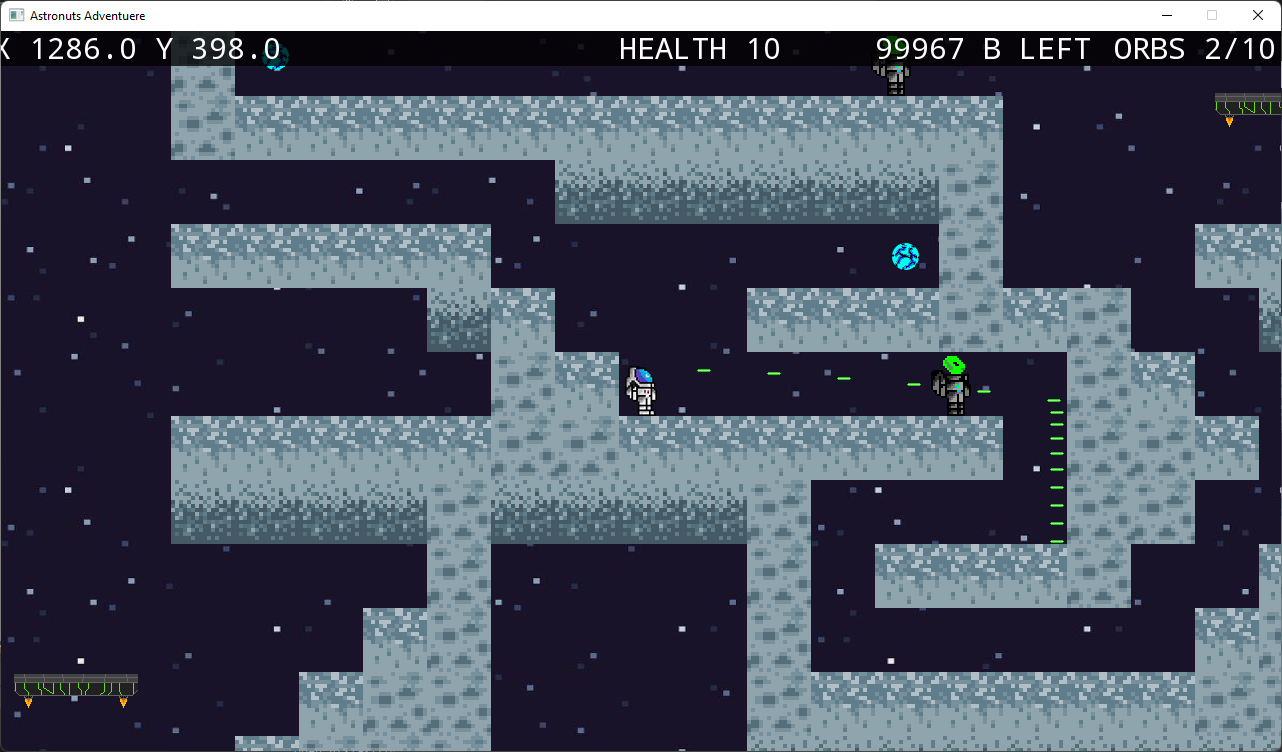
\includegraphics[width=1\linewidth]{images/ss1.png}
The shooting functionality utilises the entity struct to create bullets. When a collision is detected, these bullets activate the touch function. If it collides with an entity, it will cause harm, and if it collides with the ground, it will disappear. The bullet's velocity is stored in the struct's dy variable, which uses the physics of all the other entities previously supplied and is inverted according on the player's location, for example, if the player fires towards the left, the bullet is shot from the left. The bullets are also restricted to one hundred every game and will – 1 for each shot until they reach 0, and the player will be unable to fire the laser gun unless an orb is obtained, which grants the player +5 bullets.
\lstinputlisting[language=c]{C:/Users/ru4en/OneDrive/Desktop/SpringProjectx/src/attack.c}
 
 \newpage

\subsection{Enemy (Aliens)}
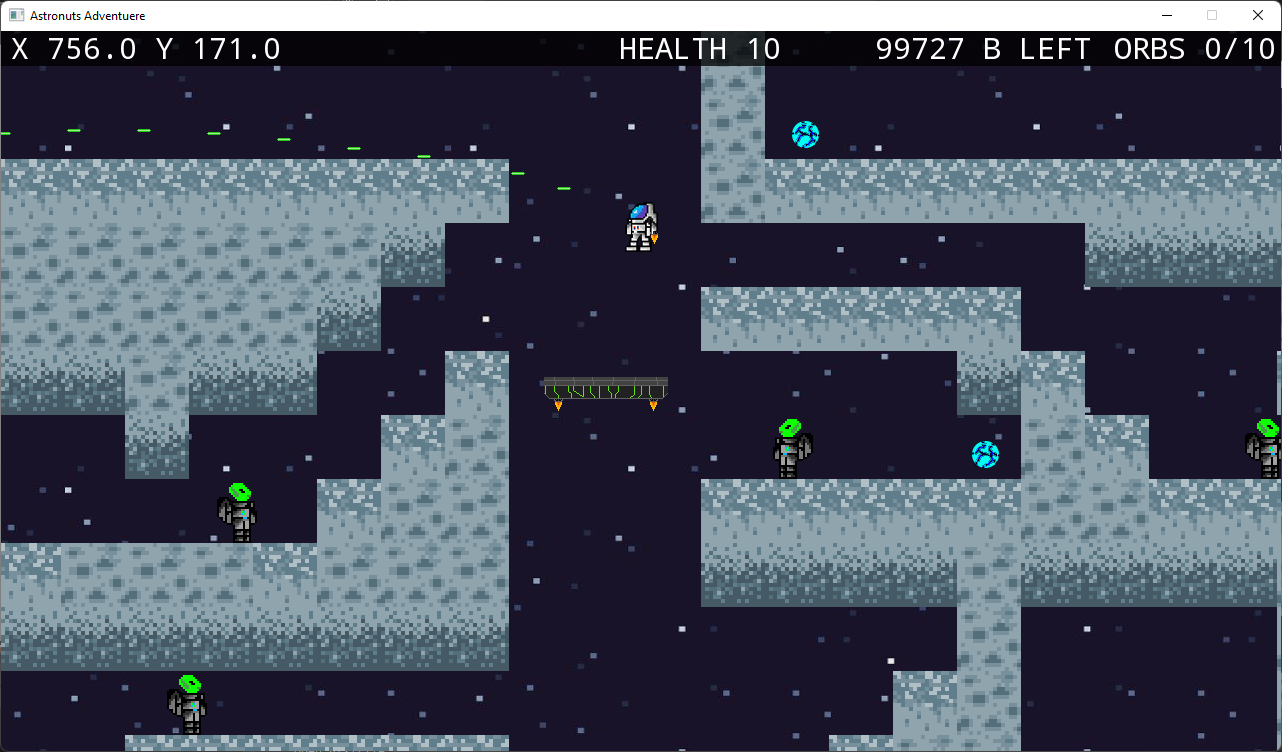
\includegraphics[width=1\linewidth]{images/ss3.png}
The aliens were designed to add a level of difficulty to the game. Alien movement from sx to ex is similar to platforms and may be set in the etntery.dat file. If the player fires at these aliens, they will receive damage, and if the player touches them, they will kill the player instantaneously. The aliens have two textures, which are kept in an array of SDL texture. It likewise made use of the same struct as the other entities. 
\lstinputlisting[language=c]{C:/Users/ru4en/OneDrive/Desktop/SpringProjectx/src/enemy.c}
  